% TeX eps-loader file generated by stoch_simul.m (Dynare).
% 06-Nov-2023 17:57:19
 
\begin{figure}[H]
\centering 
\includegraphics[width=0.80\textwidth]{directed_search/graphs/directed_search_IRF_e_ZI1}
\caption{Impulse response functions (orthogonalized shock to $e\_ZI$).}\label{Fig:IRF:e_ZI:1}
\end{figure}
 
\begin{figure}[H]
\centering 
\includegraphics[width=0.80\textwidth]{directed_search/graphs/directed_search_IRF_e_ZI2}
\caption{Impulse response functions (orthogonalized shock to $e\_ZI$).}\label{Fig:IRF:e_ZI:2}
\end{figure}
 
\begin{figure}[H]
\centering 
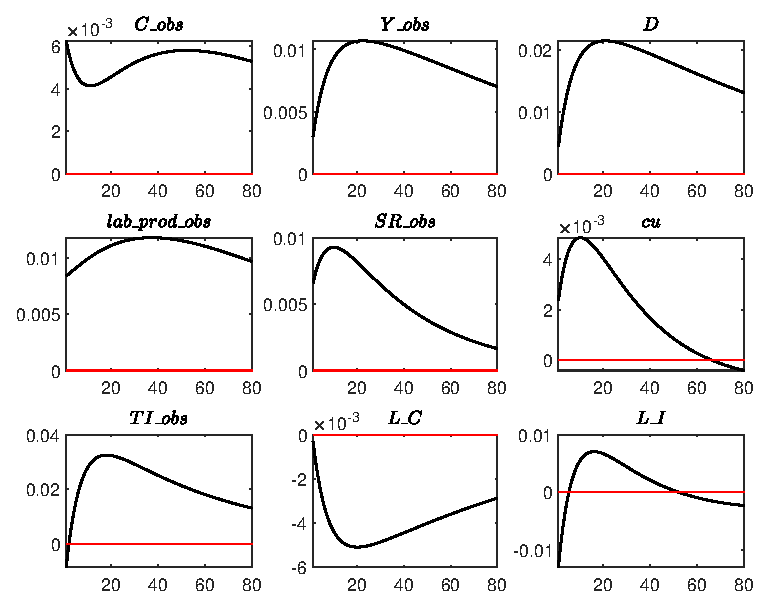
\includegraphics[width=0.80\textwidth]{directed_search/graphs/directed_search_IRF_e_Z1}
\caption{Impulse response functions (orthogonalized shock to $e\_Z$).}\label{Fig:IRF:e_Z:1}
\end{figure}
 
\begin{figure}[H]
\centering 
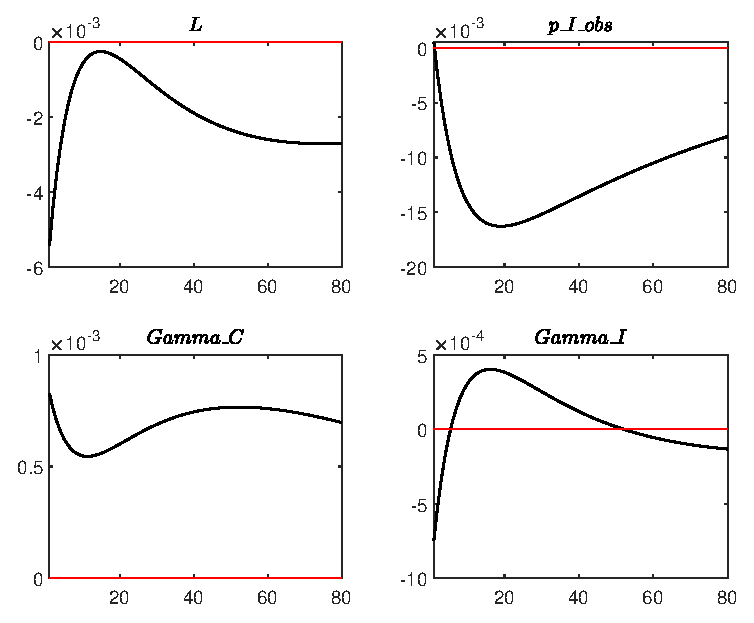
\includegraphics[width=0.80\textwidth]{directed_search/graphs/directed_search_IRF_e_Z2}
\caption{Impulse response functions (orthogonalized shock to $e\_Z$).}\label{Fig:IRF:e_Z:2}
\end{figure}
 
\begin{figure}[H]
\centering 
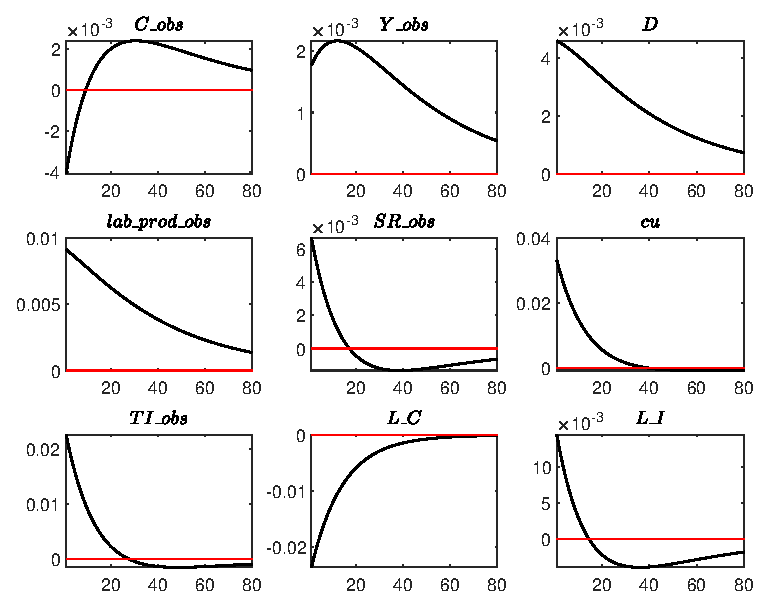
\includegraphics[width=0.80\textwidth]{directed_search/graphs/directed_search_IRF_e_shop1}
\caption{Impulse response functions (orthogonalized shock to $e\_shop$).}\label{Fig:IRF:e_shop:1}
\end{figure}
 
\begin{figure}[H]
\centering 
\includegraphics[width=0.80\textwidth]{directed_search/graphs/directed_search_IRF_e_shop2}
\caption{Impulse response functions (orthogonalized shock to $e\_shop$).}\label{Fig:IRF:e_shop:2}
\end{figure}
 
\begin{figure}[H]
\centering 
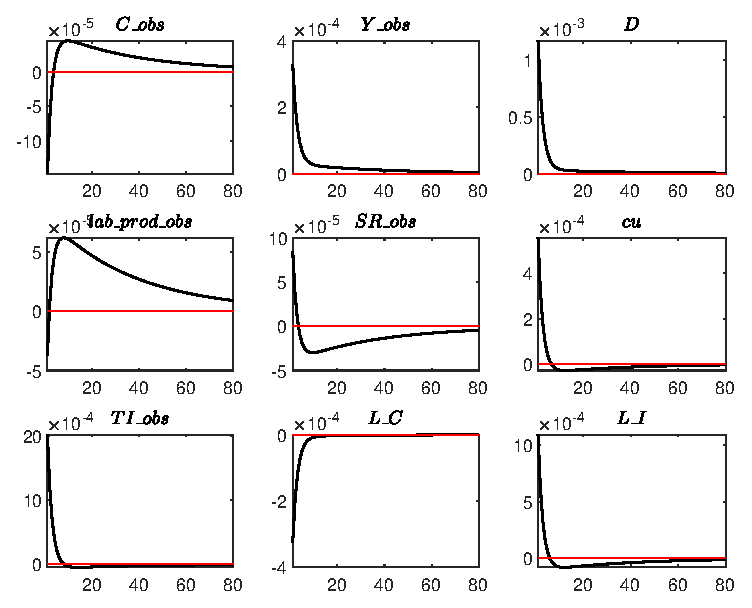
\includegraphics[width=0.80\textwidth]{directed_search/graphs/directed_search_IRF_e_zeta1}
\caption{Impulse response functions (orthogonalized shock to $e\_zeta$).}\label{Fig:IRF:e_zeta:1}
\end{figure}
 
\begin{figure}[H]
\centering 
\includegraphics[width=0.80\textwidth]{directed_search/graphs/directed_search_IRF_e_zeta2}
\caption{Impulse response functions (orthogonalized shock to $e\_zeta$).}\label{Fig:IRF:e_zeta:2}
\end{figure}
 
\begin{figure}[H]
\centering 
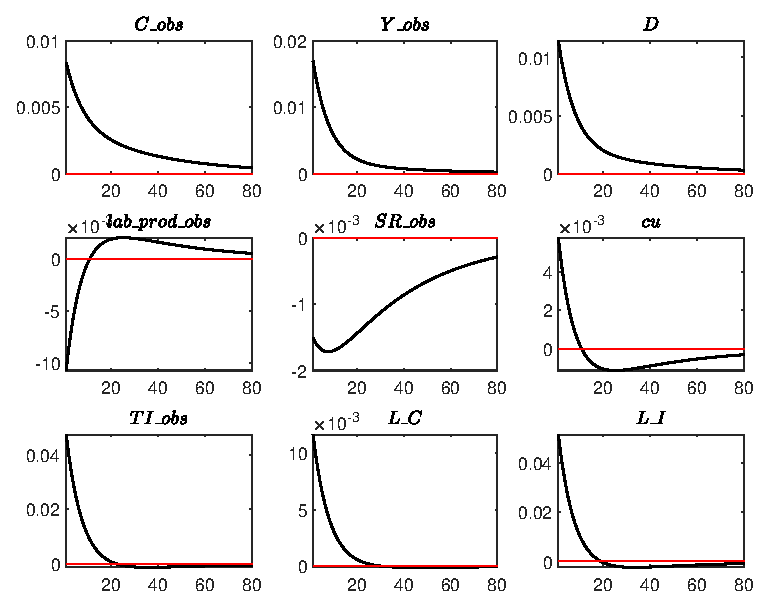
\includegraphics[width=0.80\textwidth]{directed_search/graphs/directed_search_IRF_e_chi1}
\caption{Impulse response functions (orthogonalized shock to $e\_chi$).}\label{Fig:IRF:e_chi:1}
\end{figure}
 
\begin{figure}[H]
\centering 
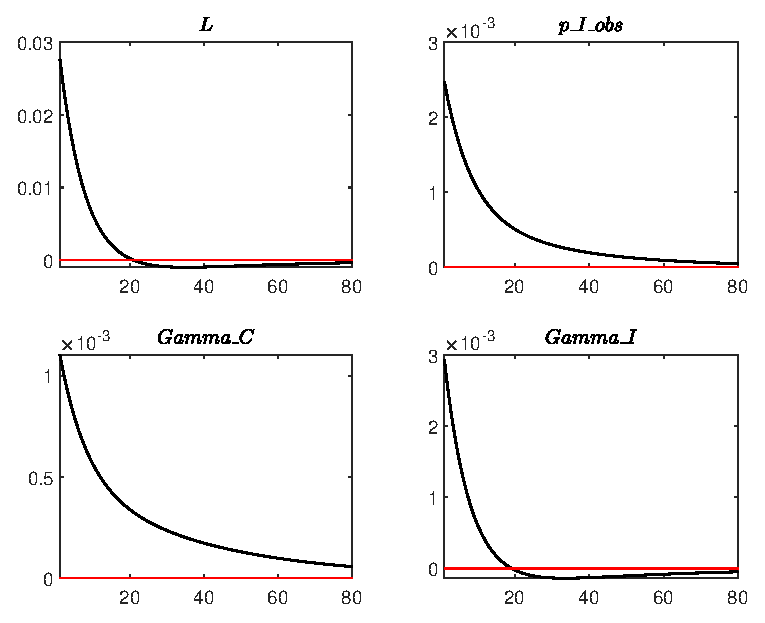
\includegraphics[width=0.80\textwidth]{directed_search/graphs/directed_search_IRF_e_chi2}
\caption{Impulse response functions (orthogonalized shock to $e\_chi$).}\label{Fig:IRF:e_chi:2}
\end{figure}
 
 
% End Of TeX file. 
